\let\negmedspace\undefined
\let\negthickspace\undefined
\documentclass[journal]{IEEEtran}
\usepackage[a5paper, margin=10mm, onecolumn]{geometry}
%\usepackage{lmodern} % Ensure lmodern is loaded for pdflatex
\usepackage{tfrupee} % Include tfrupee package

\setlength{\headheight}{1cm} % Set the height of the header box
\setlength{\headsep}{0mm}     % Set the distance between the header box and the top of the text

\usepackage{gvv-book}
\usepackage{gvv}
\usepackage{cite}
\usepackage{amsmath,amssymb,amsfonts,amsthm}
\usepackage{algorithmic}
\usepackage{graphicx}
\usepackage{textcomp}
\usepackage{xcolor}
\usepackage{txfonts}
\usepackage{listings}
\usepackage{enumitem}
\usepackage{mathtools}
\usepackage{gensymb}
\usepackage{comment}
\usepackage[breaklinks=true]{hyperref}
\usepackage{tkz-euclide} 
\usepackage{listings}
% \usepackage{gvv}                                        
\def\inputGnumericTable{}                                 
\usepackage[latin1]{inputenc}                                
\usepackage{color}                                            
\usepackage{array}                                            
\usepackage{longtable}                                       
\usepackage{calc}                                             
\usepackage{multirow}                                         
\usepackage{hhline}                                           
\usepackage{ifthen}                                           
\usepackage{lscape}
\usepackage{circuitikz}


\renewcommand{\thefigure}{\theenumi}
\renewcommand{\thetable}{\theenumi}
\setlength{\intextsep}{10pt} % Space between text and floats


\numberwithin{equation}{enumi}
\numberwithin{figure}{enumi}
\renewcommand{\thetable}{\theenumi}


% Marks the beginning of the document
\begin{document}
\bibliographystyle{IEEEtran}
\vspace{3cm}

\title{GATE CS 2008}
\author{EE25BTECH11011 - Banavathu Navya}
\maketitle

% (add your content here)
\begin{center}
 \textbf{Q.1 - Q.20 Carry One Mark Each.}
\end{center}
\begin{enumerate}
    \item $\lim_{x \to \infty}\frac{x - \sin x}{x+ \cos x}$ equals
\begin{multicols}{4}
\begin{enumerate}
    \item $1$
    \item $-1$
    \item $\infty$
    \item $0$
\end{enumerate}
\end{multicols}
\hfill $\brak{GATE\ CS\  2008}$

\item If $P$, $Q$, $R$ are subsets of the universal set $U$,then  $(P \cap Q \cap R) \cup (P^c \cap Q \cap R) \cup Q^c \cup R^C$ is:
\begin{enumerate} 
\begin{multicols}{4}
    \item $Q^c \cup R^c$
    \item $P \cup Q^c \cup R^c$
    \item $P^c \cup Q^c \cup R^c$
    \item $U$
\end{multicols}
\end{enumerate}
\hfill $\brak{GATE\ CS\  2008}$

\item The following system of equations
$
\begin{aligned}
x_1 + x_2 + 2x_3 &= 1 \\
x_1 + 2x_2 + 3x_3 &= 2 \\
x_1 + 4x_2 + \alpha x_3 &= 4
\end{aligned} $
has a unique solution. The only possible value(s) for \(\alpha\) is/are:
\begin{enumerate}  
\begin{multicols}{2}
    \item $0$ 
    \item either $0$ or $1$ 
    \item one of $0$, $1$ or $-1$
    \item any real number
\end{multicols}
\end{enumerate}
\hfill $\brak{GATE\ CS\  2008}$

\item In the IEEE floating point representation the hexadecimal value 0x00000000 corresponds to
 \begin{enumerate} 
\begin{multicols}{2}
    \item The normalized value $2^{-127}$
    \item The normalized value $2^{-126}$
    \item The normalized value $+0$
    \item The special value $+0$
\end{multicols}
\end{enumerate}
\hfill $\brak{GATE\ CS\  2008}$

\item In the Karnaugh map shown below, \(X\) denotes a don't care term.  
What is the minimal form of the function represented by the Karnaugh map?
\begin{figure}[H]
    \centering
    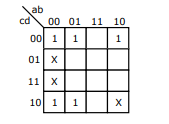
\includegraphics[width=0.5\columnwidth]{figs/fig1.png}
    \caption{Karnaugh map}
    \label{fig:1}
   \end{figure}
\begin{enumerate}
\begin{multicols}{4}
    \item $\overline{b} \cdot d + a \cdot \overline{d}$
    \item $a \cdot \overline{b} + \overline{b} \cdot d + a \cdot b \cdot \overline{d}$
    \item $b \cdot d + a \cdot \overline{d}$
    \item $a \cdot \overline{b} + \overline{b} \cdot d + \overline{a} \cdot d$
\end{multicols}
\end{enumerate}
\hfill $\brak{GATE\ CS\  2008}$

\item Let $r$ denote number system radix. The only value(s) of $r$ that satisfy the equation $\sqrt{121_r}= 11_r$ is / are 
\begin{enumerate}
\begin{multicols}{2}
    \item decimal $10$
    \item decimal $11$
    \item decimal $10$ and $11$
    \item any value $>2$
\end{multicols}
\end{enumerate}
\hfill $\brak{GATE\ CS\  2008}$

\item The most efficient algorithm for finding the number of connected components in an undirected graph on n vertices and m edges has time complexity 
\begin{enumerate} 
\begin{multicols}{4}
    \item $\theta(n)$ 
    \item $\theta(m)$
    \item $\theta(m+n)$
    \item $\theta(mn)$
\end{multicols}
\end{enumerate}
\hfill $\brak{GATE\ CS\  2008}$

\item Given $f_1$, $f_3$ and $f$ in canonical sum of products form (in decimal) for the circuit 
\begin{figure}[H]
    \centering
    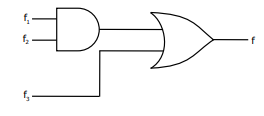
\includegraphics[width=0.5\columnwidth]{figs/fig2.png}
    \caption{Logic circuit for functions $f_1$, $f_2$, and $f_3$ in canonical sum of products form.}
    \label{fig:2}
   \end{figure}
     $f_1 = \Sigma m(4,5,6,7,8)$\\
     $f_3 = \Sigma m(1,6,15)$\\
     $f= \Sigma m(1,6,15)$\\
     then $f_2$ is
\begin{enumerate} 
\begin{multicols}{4}
    \item $\Sigma m(4,6)$
    \item $\Sigma m(4,8)$
    \item $\Sigma m(6,8)$
    \item $\Sigma m(4,6,8)$
\end{multicols}
\end{enumerate}
\hfill $\brak{GATE\ CS\  2008}$

\item Which of the following is true for the language $\{a^p \mid p \text{ is a prime}\}$
 \begin{enumerate}
    \item It is not accepted by a Turing Machine 
    \item It is regular but not context-free 
    \item It is context-free but not regular 
    \item It is neither regular nor context-free, but accepted by a Turing machine 
\end{enumerate}
\hfill $\brak{GATE\ CS\  2008}$

\item Which of the following are decidable? 
\begin{enumerate} 
    \item Whether the intersection of two regular languages is infinite  
    \item Whether a given context-free language is regular  
    \item  Whether two push-down automata accept the same language 
    \item Whether a given grammar is context-free 
\end{enumerate}
\begin{enumerate}
\begin{multicols}{4}
   \item I and II
    \item I and IV
    \item II and III
    \item II and IV
\end{multicols}
\end{enumerate}
\hfill $\brak{GATE\ CS\  2008}$

\item Which of the following describes a handle (as applicable to LR-parsing) 
appropriately? 
\begin{enumerate}
    \item It is the position in a sentential form where the next shift or reduce operation will occur
    \item It is non-terminal whose production will be used for reduction in the next step 
    \item It is a production that may be used for reduction in a future step along with a position in the sentential form where the next shift or reduce operation will occur
    \item It is the production p that will be used for reduction in the next step along with a position in the sentential form where the right hand side of the production may be found 
\end{enumerate}
\hfill $\brak{GATE\ CS\  2008}$

\item Some code optimizations are carried out on the intermediate code because 
   \begin{enumerate}
   \item They enhance the portability of the compiler to other target processors 
   \item Program analysis is more accurate on intermediate code than on machine code
   \item The information from dataflow analysis cannot otherwise be used for optimization
   \item The information from the front end cannot otherwise be used for optimization
\end{enumerate}
\hfill $\brak{GATE\ CS\  2008}$

\item If $L$ and $\overline{L}$ are recursively enumerable then $L$ is
\begin{enumerate} 
\begin{multicols}{2}
    \item regular
    \item context-free 
    \item context-sensitive
    \item  recursive
\end{multicols}
\end{enumerate}
\hfill $\brak{GATE\ CS\  2008}$

\item What is the maximum size of data that the application layer can pass on to the TCP layer below?
\begin{enumerate} 
\begin{multicols}{2}
   \item Any size
   \item $2^{16}$ bytes-size of TCP header 
   \item  $2^{16}$ bytes
   \item $1500$ bytes 
\end{multicols}
\end{enumerate}
\hfill $\brak{GATE\ CS\  2008}$

\item Which of the following tuple relational calculus expression(s) is/are equivalent to $\forall t \in r \left(P(t)\right)$ ?
\begin{enumerate} 
   \item $\neg \exists t \in r \left(P(t)\right)$
   \item $\exists t \notin r \left(P(t)\right)$
   \item $\neg \exists t \in r \left (\neg P(t)\right)$
   \item $ \exists t \notin r \left (\neg P(t)\right)$
\end{enumerate}
\begin{enumerate}
\begin{multicols}{4}
    \item I only
    \item II only
    \item III only
    \item III and IV
\end{multicols}
\end{enumerate}
\hfill $\brak{GATE\ CS\  2008}$

\item A clustering index is defined on the fields which are of type
\begin{enumerate} 
\begin{multicols}{2}
    \item  non-key and ordering
    \item  non-key and non-ordering
    \item key and ordering
    \item key and non-ordering
\end{multicols}
\end{enumerate}
\hfill $\brak{GATE\ CS\  2008}$

\item Which of the following system calls results in the sending of SYN packets? 
\begin{enumerate} 
\begin{multicols}{4}
    \item socket
    \item bind
    \item listen
    \item connect
\end{multicols}
\end{enumerate}
\hfill $\brak{GATE\ CS\  2008}$

\item Which combination of the integer variables x, y and z makes the variable a get the value 4 in the following expression? 
    
$a = (x>y)?((x>z)?x:z):((y>z)?y:z)$

\begin{enumerate}
\begin{multicols}{2}
   \item $x=3,y=4,z=2$
   \item $x=6,y=5,z=3$
   \item $x=6,y=3,z=5$
   \item $x=5,y=4,z=5$
\end{multicols}
\end{enumerate}
\hfill $\brak{GATE\ CS\  2008}$

\item The Breadth First Search algorithm has been implemented using the queue data structure. One possible order of visiting the nodes of the following graph is
\begin{figure}[H]
\centering
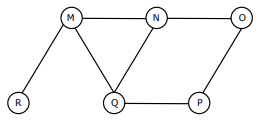
\includegraphics[width=0.5\columnwidth]{figs/fig3.png}
\caption{Graph}
\label{fig:3}
\end{figure}
 \begin{enumerate}
\begin{multicols}{4}
    \item  MNOPQR
    \item NQMPOR
    \item QMNPRO
    \item  QMNPOR
\end{multicols}
\end{enumerate}
\hfill $\brak{GATE\ CS\  2008}$

\item The data blocks of a very large file in the Unix file system are allocated using
\begin{enumerate}
    \item contiguous allocation
    \item  linked allocation 
    \item indexed allocation 
    \item an extension of indexed allocation 
\end{enumerate}
\hfill $\brak{GATE\ CS\  2008}$
 

\begin{center}
\textbf{Q. 21 -- Q. 75 carry one mark each}.
\end{center}
\item The minimum number of equal length subintervals needed to approximate $\int_{1}^{2} x e^x \,dx$ to an accuracy of at least $\frac{1}{3}times 10^{-6}$ using the trapezoidal rule is
\begin{enumerate}
\begin{multicols}{4}
    \item $1000$e
    \item $1000$
    \item $100$e
    \item $100$
\end{multicols}
\end{enumerate}
\hfill $\brak{GATE\ CS\  2008}$

\item The Newton-Raphson iteration $x_{n+1}=\frac{1}{2}(x_n+\frac{R}{x_n})$ can be used to compute the 
\begin{enumerate}
\begin{multicols}{2}
\item  square of R
    \item reciprocal of R
    \item square root of R
    \item  logarithm of R
\end{multicols}
\end{enumerate}
\hfill $\brak{GATE\ CS\  2008}$

\item  Which of the following statements is true for every planar graph on $n$ vertices? 
\begin{enumerate}
    \item  The graph is connected
    \item  The graph is Eulerian
    \item  The graph has a vertex-cover of size at most $3$n/$4$
    \item The graph has an independent set of size at least n/$3$
\end{enumerate}
\hfill $\brak{GATE\ CS\  2008}$
 

\item Let \[ P = \sum\nolimits_{\substack{1 \le i \le 2k \\ i\ \text{odd}}} i \quad\text{and}\quad Q = \sum\nolimits_{\substack{1 \le i \le 2k \\ i\ \text{even}}} i \]where \(k\) is a positive integer. Then 
\begin{enumerate}
\begin{multicols}{4}
    \item   P=Q-K
    \item  P=Q+K
    \item  P=Q
    \item  P=Q+$2$K
\end{multicols}
\end{enumerate}
\hfill $\brak{GATE\ CS\  2008}$

\item A point on a curve is said to be an extremum if it is a local minimum or a local maximum. The number of distinct extrema for the curve $3x^4-16x^3+24x^2+37$ is 
\begin{enumerate}
\begin{multicols}{4}
    \item  $0$
    \item  $1$
    \item  $2$
    \item  $3$
\end{multicols}
\end{enumerate}
\hfill $\brak{GATE\ CS\  2008}$

\item If P, Q, R are Boolean variables, then \\
$(P+\overline{Q})(P.\overline{Q}+P.R)(\overline{P}.\overline{R}+\overline{Q})$\\
Simplifies  to
\begin{enumerate}
\begin{multicols}{4}
    \item $P.\overline{Q}$
    \item $P.\overline{R}$
    \item $P.\overline{Q}+R$
    \item $P.\overline{R}+Q$
\end{multicols}
\end{enumerate}
\hfill $\brak{GATE\ CS\  2008}$

\item Aishwarya studies either computer science or mathematics everyday. If she studies computer science on a day, then the probability that the studies mathematics the next day is $0.6$. If she studies mathematics on a day, then the probability that the studies computer science the next day is $0.4$. Given that Aishwarya studies computer science on Monday, what is the probability that she studies computer science on Wednesday?
\begin{enumerate} 
\begin{multicols}{4}
    \item $0.24$
    \item $0.36$
    \item $0.4$
    \item $0.6$
\end{multicols}
\end{enumerate}
\hfill $\brak{GATE\ CS\  2008}$

\item How many of the following matrices have an eigenvalue $1$?
$
\myvec{1 & 0 \\
0 & 0}
\myvec{1 & 1 \\
0 & 1}
\myvec{1 & -1 \\
0 & 1}
\myvec{-1 & 0 \\
0 & -1}
$

\begin{enumerate}
\begin{multicols}{4}
   \item one
   \item two
   \item three
   \item four
\end{multicols}
\end{enumerate}
\hfill $\brak{GATE\ CS\  2008}$

\item Let $X$ be a random variable following normal distribution with mean $+1$ and variance $4$. Let $Y$ be another normal variable with mean $-1$ and variance unknown. If $P(X\leq-1)= P( Y\geq 2)$ , the standard deviation of $Y$ is 
\begin{enumerate}
\begin{multicols}{4}
   \item $3$
   \item $2$
   \item $\sqrt{2}$
   \item $1$
\end{multicols} 
\end{enumerate}
\hfill $\brak{GATE\ CS\  2008}$

\item Let fsa and pda be two predicates such that \texttt{fsa}(x) means 
$x$ is a finite state automaton, and \texttt{pda}(y) means $x$ is a pushdown automaton.  
Let equivalent be another predicate such that equivalent $(a,b)$means that $a$ and $b$ are equivalent.\\  
Which of the following first order logic statements represents the following:\\

Each finite state automaton has an equivalent pushdown automaton

\begin{enumerate}
\item $(\forall x \ \texttt{fsa}(x)) \Rightarrow (\exists y \ \texttt{pda}(y) \land \texttt{equivalent}(x,y))$
\item  $ \neg \forall y  (\exists x  \texttt{fsa}(x) \Rightarrow \texttt{pda}(y) \land \texttt{equivalent}(x,y))$
\item $\forall x \ \exists y \ (\texttt{fsa}(x) \land   \texttt{pda}(y) \land \texttt{equivalent}(x,y))$
\item $\forall x \ \exists y \ (\texttt{fsa}(y) \land \texttt{pda}(x) \land \texttt{equivalent}(x,y))$
\end{enumerate}
\hfill $\brak{GATE\ CS\  2008}$
 

\item $P$ and $Q$ are two propositions. Which of the following logical expressions are
equivalent? 
\begin{enumerate}   
   \item \quad $P \lor \neg Q  $  
   \item \quad $\lnot (\neg P \land Q) $  
   \item \quad $(P \land Q) \lor ( P \land \lnot Q) \lor (\neg P \land \neg Q)$  
   \item \quad $(P \land Q) \lor ( P \land \lnot Q) \lor (\neg P \land  Q)$  
\end{enumerate}
\begin{enumerate}
\begin{multicols}{2}
   \item Only I and II
   \item Only I, II and III
   \item Only I, II and IV
   \item All of I, II, III and IV
\end{multicols}
\end{enumerate}
\hfill $\brak{GATE\ CS\  2008}$

\item For a magnetic disk with concentric circular tracks, the seek latency is not linearly
proportional to the seek distance due to 
\begin{enumerate}
   \item non-uniform distribution of requests
   \item  arm starting and stopping inertia
   \item higher capacity of tracks on the periphery of the platter
   \item use of unfair arm scheduling policies
\end{enumerate}
\hfill $\brak{GATE\ CS\  2008}$
 

\item Which of the following is/are true of the auto-increment addressing mode? 
\begin{enumerate}   
   \item It is useful in creating self-relocating code
   \item  If it is included in an Instruction Set Architecture, then an additional ALU is required for effective address calculation
   \item The amount of increment depends on the size of the data item accessed 
\end{enumerate}

 \begin{enumerate}
\begin{multicols}{4}
\item  I only
\item  II only
 \item III only
 \item II and III only 
\end{multicols}
 \end{enumerate}
\hfill $\brak{GATE\ CS\  2008}$

\item Which of the following must be true for the RFE (Return From Exception) instruction on a general purpose processor?
\begin{enumerate}   
   \item It must be a trap instruction
   \item It must be a privileged instruction
   \item An exception cannot be allowed to occur during execution of an RFE instruction
\end{enumerate}
\begin{enumerate}
\begin{multicols}{2}
   \item  I only
   \item  II only
   \item I and II  only
   \item I,II and III only 
\end{multicols}
\end{enumerate}
\hfill $\brak{GATE\ CS\  2008}$

\item For inclusion to hold between two cache levels $L1$ and $L2$ in a multi-level cache hierarchy, which of the following are necessary?
\begin{enumerate}   
   \item $L1$ must be a write-through cache
   \item $L2$ must be a write-through cache
   \item The associativity of L2 must be greater than that of $L1$
   \item The $L2$ cache must be at least as large as the $L1$ cache
\end{enumerate}

 \begin{enumerate}
\begin{multicols}{2}
   \item  IV only
   \item  I and IV only
   \item  I, II and IV only
   \item  I, II, III and IV
\end{multicols}
\end{enumerate}
\hfill $\brak{GATE\ CS\  2008}$

\item Which of the following are NOT true in a pipelined processor?
\begin{enumerate}   
   \item Bypassing can handle all RAW hazards 
   \item Register renaming can eliminate all register carried WAR hazards
   \item Control hazard penalties can be eliminated by dynamic branch prediction
\end{enumerate}

 \begin{enumerate}
\begin{multicols}{4}
   \item  I and II only
   \item  I and III only
   \item  II and III only
   \item  I, II and III
\end{multicols}
\end{enumerate}
\hfill $\brak{GATE\ CS\  2008}$

\item The use of multiple register windows with overlap causes a reduction in the number of memory accesses for 
\begin{enumerate}   
   \item Function locals and parameters
   \item Register saves and restores
   \item Instruction
\end{enumerate}

 \begin{enumerate}
\begin{multicols}{4}
   \item  I only
   \item  II only
   \item  III only
   \item  I, II and III
\end{multicols}
\end{enumerate}
\hfill $\brak{GATE\ CS\  2008}$

\item In an instruction execution pipeline, the earliest that the data TLB (Translation Lookaside Buffer) can be accessed is 
\begin{enumerate}
   \item Before effective address calculation has started
   \item During effective address calculation
   \item After effective address calculation has completed
   \item After data cache lookup has completed
\end{enumerate}
\hfill $\brak{GATE\ CS\  2008}$
 

\item Consider the following functions:
\begin{align*}
f(n) = 2^n \\
\quad g(n) = n!\\
\quad h(n) = n^{\log n}
\end{align*}
Which of the following statements about the asymptotic behaviour of $f(n)$, $g(n)$ and $h(n)$ is true?
\begin{enumerate}
\begin{multicols}{2}
    \item[(A)] $f(n) = O(g(n));\ g(n) = O(h(n))$
    \item[(B)] $f(n) = \Omega(g(n));\ g(n) = O(h(n))$
    \item[(C)] $g(n) = O(f(n));\ h(n) = O(f(n))$
    \item[(D)] $h(n) = O(f(n));\ g(n) = \Omega(f(n))$
\end{multicols}
\end{enumerate}
\hfill $\brak{GATE\ CS\  2008}$

\item The minimum number of comparisons required to determine if an integer appears more than $n/2$ times in a sorted array of n integers is
\begin{enumerate}
\begin{multicols}{4}
   \item $\theta(n)$
   \item $\theta(logn)$
   \item $\theta(log^*n)$
   \item $\theta(1)$
\end{multicols}
\end{enumerate}
\hfill $\brak{GATE\ CS\  2008}$

\item A B-tree of order $4$ is built from scratch by $10$ successive insertions. What is the maximum number of node splitting operations that may take place?
\begin{enumerate} 
\begin{multicols}{4}
   \item $3$
   \item $4$
   \item $5$
   \item $6$
\end{multicols}
\end{enumerate}
\hfill $\brak{GATE\ CS\  2008}$

\item G is a graph on n vertices and $2n-2$ edges. The edges of G can be partitioned into two edge-disjoint spanning trees. Which of the following is NOT true for G?
\begin{enumerate}
   \item For every subset of $k$ vertices, the induced subgraph has at most $2k-2$ edges 
   \item The minimum cut in G has at least two edges
   \item There are two edge-disjoint paths between every pair of vertices 
   \item There are two vertex-disjoint paths between every pair of vertices 
\end{enumerate}
\hfill $\brak{GATE\ CS\  2008}$
 
\item Consider the Quicksort algorithm. Suppose there is a procedure for finding a pivot element which splits the list into two sub-lists each of which contains at least one-fifth of the elements. Let T(n) be the number of comparisons required to sort n elements. Then
\begin{enumerate} 
\begin{multicols}{2}
    \item $T(n) \leq 2T(n/5) + n$
    \item $T(n) \leq T(n/5) + T(4n/5) + n$
    \item $T(n) \leq 2T(4n/5) + n$
    \item $T(n) \leq 2T(n/2) + n$
\end{multicols}
\end{enumerate}
\hfill $\brak{GATE\ CS\  2008}$

\item The subset-sum problem is defined as follows: Given a set S of n positive integers and a positive integer W, determine whether there is a subset of S Whose elements sum to W. 
An algorithm Q solves this problem in $O(nW)$ time. Which of the following
statements is false? 

\begin{enumerate}
   \item Q solves the subset-sum problem in polynomial time when the input is
encoded in unary
   \item  Q solves the subset-sum problem in polynomial time when the input is encoded in binary
   \item The subset sum problem belongs to the class NP
   \item The subset sum problem is NP-h
\end{enumerate}
\hfill $\brak{GATE\ CS\  2008}$
 

\item
\begin{figure}[H]
  \centering
  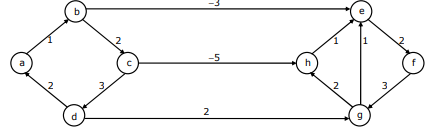
\includegraphics[width=0.5\columnwidth]{figs/fig4.png}
  \caption{Graph for Dijkstra's algorithm}
  \label{fig:4}
\end{figure}

 Dijkstra's single source shortest path algorithm when run from vertex a in the above graph, computes the correct shortest path distance to 

\begin{enumerate} 
\begin{multicols}{2}
   \item only vertex a
   \item only vertex a,e,f,g,h
   \item only vertices a,b,c,d
   \item all the vertices
\end{multicols}
\end{enumerate}
\hfill $\brak{GATE\ CS\  2008}$

\item You are given the postorder traversal, $P$, of a binary search tree on the $n$ elements $1, 2,\dots,n$. You have to determine the unique binary search tree that has $P$ as its postorder traversal. What is the time complexity of the most efficient algorithm for doing this? 
\begin{enumerate}
   \item $\theta(logn)$
   \item $\theta(n)$
   \item $\theta(nlogn)$
   \item None of the above,as the tree cannot be uniquely determined 
 \end{enumerate}
 \hfill $\brak{GATE\ CS\  2008}$
  

\item We have a binary heap on n elements and wish to insert n more elements (not necessarily one after another) into this heap. The total time required for this is
\begin{enumerate} 
\begin{multicols}{4}
   \item $\theta(logn)$
   \item $\theta(n)$
   \item $\theta(nlogn)$
   \item $\theta(n^2)$
\end{multicols}
\end{enumerate}
\hfill $\brak{GATE\ CS\  2008}$

\item Which of the following statements is false?
\begin{enumerate}
   \item  Every NFA can be converted to an equivalent DFA 
   \item Every non-deterministic Turing machine can be converted to an equivalent deterministic Turing machine 
   \item Every regular language is also a context-free language 
   \item Every subset of a recursively enumerable set is recursive
\end{enumerate}
\hfill $\brak{GATE\ CS\  2008}$
 

\item  Given below are two finite state automata ($\rightarrow$ indicates the start state and $F$ indicates a final state):
\begin{figure}[H]
    \centering
    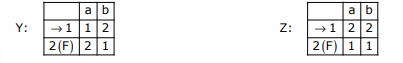
\includegraphics[width=0.5\columnwidth]{figs/fig5.png}
    \caption{two finite state automata}
    \label{figs:5}
\end{figure}

Which of the following represents the product automaton $X = Y \times Z$?
\begin{figure}[H]
    \centering
    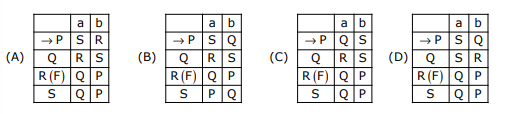
\includegraphics[width=0.5\columnwidth]{figs/fig6.png}
    \caption{Product automaton}
    \label{fig:6}
\end{figure}
\hfill $\brak{GATE\ CS\  2008}$
 

\item Which of the following statements are true?
\begin{enumerate}  
   \item Every left-recursive grammar can be converted to a right-recursive grammar and vice-versa.
   \item All $\varepsilon$-productions can be removed from any context-free grammar by suitable transformations.
   \item The language generated by a context-free grammar all of whose productions are of the form $X\to w$ or $X\to wY$ (where $w$ is a string of terminals and $Y$ is a non-terminal) is always regular.
   \item The derivation trees of strings generated by a context-free grammar in Chomsky Normal Form are always binary trees.
\end{enumerate}

 \begin{enumerate}
\begin{multicols}{2}
   \item I, II, III and IV
   \item II, III and IV only
   \item I, III and IV only
   \item I, II and IV only
\end{multicols}
\end{enumerate}
\hfill $\brak{GATE\ CS\  2008}$

\item Match the following:

\begin{tabular}{|p{5cm}|p{7cm}|}
\hline
E. Checking that identifiers are declared before their use 
& $L = \{ a^n b^m c^n d^m \mid n \geq 1,\; m \geq 1 \}$ \\
\hline
F. Number of formal parameters in the declaration of a function agrees with the number of actual parameters in use of that function 
& $X \rightarrow X b X \;\mid\; X c X \;\mid\; d X f \;\mid\; g$ \\
\hline
G. Arithmetic expressions with matched pairs of parentheses 
& $L = \{ w c w \mid w \in (a \mid b)^* \}$ \\
\hline
H. Palindromes 
& $X \rightarrow b X b \;\mid\; c X c \;\mid\; e$ \\
\hline
\end{tabular}

\begin{enumerate}
\begin{multicols}{2}
    \item E-P, F-R, G-Q, H-S
    \item E-R, F-P, G-S, H-Q
    \item E-R, F-P, G-Q, H-S
    \item E-P, F-R, G-S, H-Q
\end{multicols}
\end{enumerate}
\hfill $\brak{GATE\ CS\  2008}$

\item Match the following NFAs with the regular expressions they correspond to 
\begin{figure}[H]
    \centering
    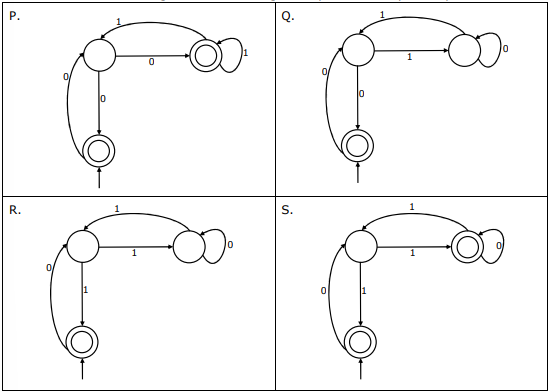
\includegraphics[width=0.5\columnwidth]{figs/fig7.png}
    \caption{NFA's}
    \label{fig:7}
\end{figure}
\begin{center}
\begin{enumerate}
    \item $\epsilon + 0(01^{*}1 + 00)^{*}01^{*}$
    \item $\epsilon + 0(10^{*}1 + 00)^{*}0$
    \item $\epsilon + 0(01^{*}1 + 10)^{*}1$
    \item $\epsilon + 0(10^{*}1 + 10)^{*}10^{*}$
\end{enumerate}
\end{center}
\begin{enumerate}
\begin{multicols}{2}
    \item[(A)] P $\rightarrow$ 2, Q $\rightarrow$ 1, R $\rightarrow$ 3, S $\rightarrow$ 4
    \item[(B)] P $\rightarrow$ 1, Q $\rightarrow$ 3, R $\rightarrow$ 2, S $\rightarrow$ 4
    \item[(C)] P $\rightarrow$ 1, Q $\rightarrow$ 2, R $\rightarrow$ 3, S $\rightarrow$ 4
    \item[(D)] P $\rightarrow$ 3, Q $\rightarrow$ 2, R $\rightarrow$ 1, S $\rightarrow$ 4
\end{multicols}
\end{enumerate}
\hfill $\brak{GATE\ CS\  2008}$

\item Which of the following are regular sets?
\begin{enumerate}  
    \item $\{a^n b^2m \mid n \geq 0, m \geq 0\}$
    \item $\{a^n b^m \mid n = 2m\}$
    \item $\{a^n b^m \mid n \not= m\}$
    \item $\{xcy \mid x, y \in \{a,b\}^*\}$
\end{enumerate}

 \begin{enumerate}
\begin{multicols}{4}
    \item I and IV only
    \item I and II only
    \item I only
    \item IV only
\end{multicols}
\end{enumerate}
\hfill $\brak{GATE\ CS\  2008}$
 
\item Which of the following are true?
\begin{enumerate}  
   \item A programming language which does not permit global variables of any kind and has no nesting of procedures/functions, but permits recursion can be implemented with static storage allocation
  \item Multi-level access link (or display) arrangement is needed to arrange activation records only if the programming language being implemented has nesting of procedures/functions
  \item Recursion in programming languages cannot be implemented with dynamic storage allocation
  \item Nesting procedures/functions and recursion require a dynamic heap allocation scheme and cannot be implemented with a stack-based allocation
scheme for activation records
  \item Programming languages which permit a function to return a function as its result cannot be implemented with a stack-based storage allocation scheme for activation records
\end{enumerate}

\begin{enumerate} 
\begin{multicols}{2}
    \item II and V only
    \item I,III and IV only
    \item I, II and V only
    \item II, III and V only
\end{multicols}
\end{enumerate}
\hfill $\brak{GATE\ CS\  2008}$

\item An LALR(1) parser for a grammar G can have shift-reduce (S-R) conflicts if and only if 
\begin{enumerate}
    \item  The SLR(1) parser for G has S-R conflicts
    \item The LR(1) parser for G has S-R conflicts
    \item The LR(0) parser for G has S-R conflicts
    \item The LALR(1) parser for G has reduce-reduce conflicts
\end{enumerate}
\hfill $\brak{GATE\ CS\  2008}$
 

\item In the slow start phase of the TCP congestion control algorithm, the size of the congestion window
\begin{enumerate} 
\begin{multicols}{2}
  \item  does not increase
  \item  increases linearly
  \item increases quadratically
  \item increases exponentially
\end{multicols}
\end{enumerate}
\hfill $\brak{GATE\ CS\  2008}$

\item If a class $B$ network on the Internet has a subnet mask of $255.255.248.0,$ what is the maximum number of hosts per subnet? 
\begin{enumerate} 
\begin{multicols}{4}
   \item $1022$
   \item $1023$
   \item $2046$
   \item $2047$
\end{multicols}
\end{enumerate}
\hfill $\brak{GATE\ CS\  2008}$

\item A computer on a $10Mbps$ network is regulated by a token bucket. The token bucket is filled at a rate of $2Mbps$. It is initially filled to capacity with $16Megabits$. What is the maximum duration for which the computer can transmit at the full $10Mbps$? 
\begin{enumerate} 
\begin{multicols}{4}
  \item  $1.6$ seconds
  \item  $2$ seconds
  \item  $5$ seconds
  \item  $8$ seconds
\end{multicols}
\end{enumerate}
\hfill $\brak{GATE\ CS\  2008}$

\item A client process P needs to make a TCP connection to a server process S.Consider the following situation: the server process S executes a socket (), a bind () and a listen () system call in that order, following which it is preempted. Subsequently, the client process P executes a socket () system call followed by connect () system call to connect to the server process S. The server process has not executed any accept () system call. Which one of the following events could take place? 
\begin{enumerate}
   \item  connect ( ) system call returns successfully
   \item  connect ( ) system call blocks
   \item connect ( ) system call returns an error
   \item connect ( ) system call results in a core dump 
\end{enumerate}    
\hfill $\brak{GATE\ CS\  2008}$

\item What is printed by the following C program?
\begin{verbatim}
int f(int *x, int *py, int **ppz)     void main()
{                                     {
    int y, z;                          int c, *b, **a;
    **ppz += 1;  z = **ppz;           c = 4;b = &c; a = &b;
    *py += 2;    y = *py;              printf("%d", f(c, b, a));
        *x += 3;                          }
    return x + y + z;                  
}
\end{verbatim}

\begin{enumerate}
\begin{multicols}{4}
   \item $18$
   \item $19$
   \item $21$
   \item $22$
\end{multicols}
\end{enumerate}
\hfill $\brak{GATE\ CS\  2008}$

\item Choose the correct option to fill \texttt{?1} and \texttt{?2} so that the program below prints an input string in reverse order. Assume that the input string is terminated by a newline character.
\begin{verbatim}
void reverse(void) {
    int c;
    if ( ?1 ) reverse();
    ?2
}

int main() {
    printf("Enter Text"); printf("\n");
    reverse(); printf("\n");
}
\end{verbatim}

\begin{enumerate}
\item \texttt{?1: (getchar() != '\textbackslash n')} \\
      \texttt{?2: getchar(c);}
\item \texttt{?1: (c = getchar()) != '\textbackslash n'} \\
      \texttt{?2: getchar(c);}
\item \texttt{?1: (c != '\textbackslash n')} \\
      \texttt{?2: putchar(c);}
\item \texttt{?1: ((c = getchar()) != '\textbackslash n')} \\
      \texttt{?2: putchar(c);}
\end{enumerate}
\hfill $\brak{GATE\ CS\  2008}$
 

\item The following C function takes a single-linked list of integers as a parameter and rearranges the elements of the list. 
The function is called with the list containing the integers $1,2,3,4,5,6,7$ in the given order. 
What will be the contents of the list after the function completes execution?

\begin{verbatim}
struct node {
    int value;
    struct node *next;
};
void rearrange(struct node *list) {
    struct node *p, *q;
    int temp;
    if (!list || !list->next) return;
    p = list; 
    q = list->next;
    while (q) {
        temp = p->value;p->value = q->value; 
       q->value = temp; p = q->next;
        q=p?p->next;    
    }
}
\end{verbatim}

\begin{enumerate}
\begin{multicols}{4}
   \item $1,2,3,4,5,6,7$
   \item $2,1,4,3,6,5,7$
   \item $1,3,2,5,4,7,6$
   \item $2,3,4,5,6,7,1$
\end{multicols}
\end{enumerate}
\hfill $\brak{GATE\ CS\  2008}$

\item The P and V operations on counting semaphores, where $s$ is a counting semaphore, are defined as follows:

\begin{verbatim}
P(s): s = s - 1;
      if s < 0 then wait;

V(s): s = s + 1;
      if s <= 0 then wakeup a process waiting on s;
\end{verbatim}

Assume that $P_b$ and $V_b$, the wait and signal operations on binary semaphores, are provided. 
Two binary semaphores $x_b$ and $y_b$ are used to implement the semaphore operations $P(s)$ and $V(s)$ as follows:


P(s):   $P_b$($x_b$);\\
        s = s - 1;\\
        if (s \l 0)  \\
            $V_b$($y_b$);\\
        else $V_b$($x_b$);

V(s):   $P_b$($x_b$);\\
        s = s + 1;\\
        if (s $\leq$ 0) $V_b$($y_b$);\\ 
        $V_b$($x_b$);\\
The initial values of $x_b$ and $y_b$ are respectively:
\begin{enumerate}
\begin{multicols}{4}
    \item $0$ and $0$
    \item $0$ and $1$
    \item $1$ and $0$
    \item $1$ and $1$
\end{multicols}
\end{enumerate}
\hfill $\brak{GATE\ CS\  2008}$

\item Which of the following statements about synchronous and asynchronous I/O is
NOT true? 
\begin{enumerate}
    \item An ISR is invoked on completion of I/O in synchronous I/O but not in
asynchronous I/O
   \item In both synchronous and asynchronous I/O, an ISR (Interrupt Service Routine) is invoked after completion of the I/O
   \item A process making a synchronous I/O call waits until I/O is complete, but a
process making an asynchronous I/O call does not wait for completion of the I/O
   \item In the case of synchronous I/O, the process waiting for the completion of I/O is woken up by the ISR that is invoked after the completion of I/O 
\end{enumerate}
\hfill $\brak{GATE\ CS\  2008}$
 

\item Which of the following is NOT true of deadlock prevention and deadlock
avoidance schemes? 
\begin{enumerate}
   \item  In deadlock prevention, the request for resources is always granted if the resulting state is safe
   \item In deadlock avoidance, the request for resources is always granted if the result state is safe
   \item Deadlock avoidance is less restrictive than deadlock prevention
   \item  Deadlock avoidance requires knowledge of resource requirements a priori   
 \end{enumerate}
\hfill $\brak{GATE\ CS\  2008}$

\item A process executes the following code

$
\text{for (i = 0; i < n; i++) for ( ; ) ;}
$
The total number of child processes created is
\begin{enumerate} 
\begin{multicols}{4}
   \item  $n$
   \item  $2^{n} - 1$
   \item  $2n$
   \item  $2^{n+1} - 1$
\end{multicols}
\end{enumerate}
\hfill $\brak{GATE\ CS\  2008}$

\item A processor uses $36$-bit physical addresses and $32$-bit virtual addresses, with a page frame size of $4$~Kbytes.  
Each page table entry is of size $4$~bytes.  
A three-level page table is used for virtual to physical address translation, where the virtual address is used as follows:

\begin{itemize}
    \item Bits $30--31$ are used to index into the first level page table
    \item Bits $21--29$ are used to index into the second level page table
    \item Bits $12--20$ are used to index into the third level page table
    \item Bits $0--11$ are used as offset within the page
\end{itemize}

The number of bits required for addressing the next level page table (or page frame) in the page table entry of the first, second, and third level page tables are respectively:
\begin{enumerate} 
\begin{multicols}{4}
   \item $20$, $20$ and $20$
   \item $24$, $24$ and $24$
   \item $24$, $24$ and $20$
   \item $25$, $25$ and $24$
\end{multicols}
\end{enumerate}
\hfill $\brak{GATE\ CS\  2008}$

\item  Let $R$ and $S$ be two relations with the following schema:

$
R(P, Q, R1, R2, R3)
$
$
S(P, Q, S1, S2)
$

Where $\{P, Q\}$ is the key for both schemas. Which of the following queries are equivalent?

\begin{enumerate}  
   \item $\quad \pi_{P}(R \Join S)$
   \item $\pi_{P}(R) \Join \pi_{P}(S)$
   \item $\pi_{P}(\pi_{P,Q}(R) - (\pi_{P,Q}(S))$
   \item $\pi_{P}(\pi_{P,Q}(R)-(\pi_{P,Q}(R) - \pi_{P,Q}(S))$
\end{enumerate}
\begin{enumerate}
\begin{multicols}{4}
   \item Only I and II
   \item Only I and III
   \item Only I, II and III
   \item Only I, III and IV
\end{multicols}
\end{enumerate}
\hfill $\brak{GATE\ CS\  2008}$

\item Consider the following relational schemes for a library database: \\
{Book (Title, Author, Catalog\_no, Publisher, Year, Price)}\\
{Collection (Title, Author, Catalog\_no)}
with in the following functional dependencies:  
\begin{enumerate}  
   \item Title, Author $\rightarrow$ Catalog\_no  
   \item Catalog\_no $\rightarrow$ Title Author Publisher Year  
   \item Publisher Title Year $\rightarrow$ Price  
\end{enumerate}

Assume $\{\text{Author}, \text{Title}\}$ is the key for both schemes. Which of the following statements is true?  

\begin{enumerate}
   \item Both Book and Collection are in BCNF  
   \item Both Book and Collection are in $3$NF only  
   \item Book is in 2NF and Collection is in $3$NF  
   \item Both Book and Collection are in $2$NF only  
\end{enumerate}
\hfill $\brak{GATE\ CS\  2008}$
 

\item Consider a file of $16384$ records. Each record is $32$ bytes long and its key field is of size $6$ bytes. The file is ordered on a non-key field, and the file organization is
unspanned. The file is stored in a file system with block size $1024$ bytes, and the size of a block pointer is $10$ bytes. If the secondary index is built on the key field
of the file, and a multi-level index scheme is used to store the secondary index, the number of first-level and second-level blocks in the multi-level index are respectively
\begin{enumerate} 
\begin{multicols}{4}
    \item $8$ and $0$
    \item $128$ and $6$
    \item $256$ and $4$
    \item $512$ and $5$
\end{multicols}
\end{enumerate}
\begin{center}
\textbf{Common Data for Questions: 71, 72 and 73}  
\end{center}
Consider a machine with a 2-way set associative data cache of size $64$Kbytes and block size $16$bytes.
The cache is managed using 32-bit virtual addresses and the page size is $4$Kbytes.  
A program to be run on this machine begins as follows:  

\begin{verbatim}
double ARR[1024][1024];

int i, j;

/* Initialize array ARR to 0.0 */
for (i = 0; i < 1024; i++)
    for (j = 0; i\j < 1024; j++)
        ARR[i][j] = 0.0;
\end{verbatim}

The size of double is $8$ Bytes.  
Array ARR is located in memory starting at the beginning of virtual page \texttt{0xF000}  
and stored in row major order.  
The cache is initially empty and no pre-fetching is done.  
The only data memory references made by the program are those to array ARR \\
\item The total size of the tags in the cache directory is
\begin{enumerate} 
\begin{multicols}{4}
   \item $32$Kbits 
   \item $34$Kbits 
   \item $64$Kbits
   \item $68$Kbits 
\end{multicols}
\end{enumerate}
\hfill $\brak{GATE\ CS\  2008}$

\item Which of the following array elements has the same cache index as ARR [0] [0]?
\begin{enumerate}
\begin{multicols}{4}
   \item  ARR [0] [4] 
   \item  ARR [4] [0]
   \item  ARR [0] [5] 
   \item  ARR [5] [0] 
\end{multicols}
\end{enumerate}
\hfill $\brak{GATE\ CS\  2008}$

\item The cache hit ratio for this initialization loop is
\begin{enumerate} 
\begin{multicols}{4}
   \item 0\%  
   \item 25\%  
   \item 50\%  
   \item 75\%  
\end{multicols}
\end{enumerate}
\hfill $\brak{GATE\ CS\  2008}$

\begin{center}
\textbf{ Common Data for Questions: 74 and 75}
\end{center}

Consider the following C functions:  

\begin{verbatim}
int f1 ( int n )
{
    if ( n == 0 || n == 1 )
        return n;
    else
        return ( 2 * f1(n - 1) + 3 * f1(n - 2) );
}

int f2 ( int n )
{
    int i;
    int X[N], Y[N], Z[N];

    X[0] = Y[0] = Z[0] = 0;
    X[1] = 1;  Y[1] = 2;  Z[1] = 3;
    for (i = 2; i <= n; i++) {
        X[i] = Y[i - 1] + Z[i - 2];
        Y[i] = 2 * X[i];
        Z[i] = 3 * X[i];
    }

    return X[n];
}
\end{verbatim}

\item The running time of f1(n) and f2(n) are
\begin{enumerate}
\begin{multicols}{2}
   \item $\Theta(n)$ and $\Theta(n)$  
   \item $\Theta(2^n)$ and $\Theta(n)$  
   \item $\Theta(n)$ and $\Theta(2^n)$  
   \item $\Theta(2^n)$ and $\Theta(2^n)$  
\end{multicols}
\end{enumerate}
\hfill $\brak{GATE\ CS\  2008}$

\item F1(8) and F2(8) return the values 
\begin{enumerate}
\begin{multicols}{2}
   \item $1661$ and $1640$  
   \item $59$ and $59$  
   \item $1640$ and $1640$  
   \item $1640$ and $1661$  
\end{multicols}
\end{enumerate}
\hfill $\brak{GATE\ CS\  2008}$

\begin{center}
\textbf{Linked Answer Questions: Q.76 to 85 Carry Two Marks Each}\\
 
\textbf{Statement for Linked Answer Questions: 76 \& 77}
\end{center}
Delayed branching can help in the handling of control hazards  

\item For all delayed conditional branch instructions, irrespective of whether the condition evaluates to true or false  
\begin{enumerate}
   \item The instruction following the conditional branch instruction in memory is executed  
   \item The first instruction in the fall through path is executed  
   \item The first instruction in the taken path is executed  
   \item The branch takes longer to execute than any other instruction  
\end{enumerate}
 
\hfill $\brak{GATE\ CS\  2008}$

\item The following code is to run on a pipelined processor with one branch delay slot:  

\begin{verbatim}
I1: ADD  R2 <- R7 + R8
I2: SUB  R4 <- R5 - R6
I3: ADD  R1 <- R2 + R3
I4: STORE Memory[R4] <- R1
    BRANCH to Label if R1 == 0
\end{verbatim}

Which of the instructions I1, I2, I3 or I4 can legitimately occupy the delay slot without any other program modification?
\begin{enumerate} 
\begin{multicols}{4}
   \item I1
   \item I2  
   \item I3  
   \item I4  
\end{multicols}
\end{enumerate}
\hfill $\brak{GATE\ CS\  2008}$

\begin{center}
\textbf{Statement for Linked Answer Questions: 78 \& 79}
\end{center}
 
Let $x_n$ denote the number of binary strings of length $n$ that contain no consecutive $0$s.

\item Which of the following recurrences does $x_n$ satisfy? 
\begin{enumerate} 
\begin{multicols}{4}
   \item $x_n = 2x_{n-1}$  
   \item $x_n = x_{\lfloor n/2 \rfloor} + 1$  
   \item $x_n = x_{\lfloor n/2 \rfloor} + n$  
   \item $x_n = x_{n-1} + x_{n-2}$  
\end{multicols}
\end{enumerate}
\hfill $\brak{GATE\ CS\  2008}$

\item The value of $x_5$ is:
\begin{enumerate} 
\begin{multicols}{4}
   \item $5$  
   \item $7$  
   \item $8$  
   \item $16$  
\end{multicols}
\end{enumerate}
\hfill $\brak{GATE\ CS\  2008}$

\begin{center}
\textbf{Statement for Linked Answer Questions: 80 \& 81}
\end{center}
 
The subset-sum problem is defined as follows: Given a set of $n$ positive integers, $S = \{a_1, a_2, a_3, \dots, a_n\}$, and positive integer $W$, is there a subset of $S$ whose elements sum to $W$? A dynamic program for solving this problem uses a 2-dimensional Boolean array, $X$, with $n$ rows and $W+1$ columns.

$X[i, j], \ 1 \leq i \leq n, \ 0 \leq j \leq W$, is TRUE if and only if there is a subset of $\{a_1, a_2, \dots, a_i\}$ whose elements sum to $j$.
 

\item Which of the following is valid for $2 \leq i \leq n$ and $1 \leq j \leq W$? 
\begin{enumerate} 
\begin{multicols}{2}
   \item $X[i, j] = X[i-1, j] \lor X[i-1, j-a_i]$  
   \item $X[i, j] = X[i, j-1] \lor X[i-1, j-a_i]$  
   \item $X[i, j] = X[i-1, j] \land X[i-1, j-a_i]$  
   \item $X[i, j]=X[i-1, j-1] \land X[i-1, j-a_i]$  
\end{multicols}
\end{enumerate}
\hfill $\brak{GATE\ CS\  2008}$

\item Which entry of the array $X$, if TRUE, implies that there is a subset whose elements sum to $W$? 
\begin{enumerate} 
\begin{multicols}{4}
   \item $X[1, W]$  
   \item $X[n, 0]$  
   \item $X[n, W]$  
   \item $X[1, n]$  
\end{multicols}
\end{enumerate}
\hfill $\brak{GATE\ CS\  2008}$

\begin{center}
\textbf{Statement for Linked Answer Questions: 82 \& 83}
\end{center}
Consider the following ER diagram:
\begin{figure}[H]
    \centering
    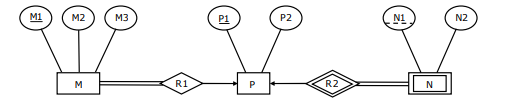
\includegraphics[width=0.5\columnwidth]{figs/fig8.png}
    \caption{ER diagram}
    \label{fig:8}
   \end{figure}

\item The minimum number of tables needed to represent M, N, P, R$1$, R$2$ is  
\begin{enumerate}
\begin{multicols}{4}
   \item $2$
   \item $3$
   \item $4$
   \item $5$
\end{multicols}
\end{enumerate}
\hfill $\brak{GATE\ CS\  2008}$

\item Which of the following is a correct attribute set for one of the tables for the correct answer to the above question?  
 \begin{enumerate}
\begin{multicols}{4}
\item $\brak{M1,M2,M3,P1}$ 
\item $\brak{M1,P1,N1,N2}$ 
\item $\brak{M1,P1,N1}$
\item $\brak{M1,P1}$ 
\end{multicols}
\end{enumerate}
\hfill $\brak{GATE\ CS\  2008}$

\begin{center}
\textbf{Statement for Linked Answer Questions: 84 \& 85}
\end{center}
Consider the following C program that attempts to locate an element $x$ in an array $Y$[ ] using binary search. The program is erroneous.

\begin{verbatim}
1.f(int Y[10], int x) {
2.    int u, j, k;
3.    i = 0, j = 9;
4.    do {
5.        k = (i + j) / 2;
6.        if (Y[k] <= k) i = k; else j = k;
7.    } while ((Y[k] != x) && (i < j));
8.    if (Y[k] == x) printf("x is in the array");
9.    else printf("x is not in the array");
10. }
\end{verbatim}
 

\item On which of the following contents of $Y$ and $x$ does the program fail?

\begin{enumerate}
    \item $Y$ is [1 2 3 4 5 6 7 8 9 10] and $x < 10$
    \item $Y$ is [1 3 5 7 9 11 13 15 17 19] and $x < 1$
    \item $Y$ is [2 2 2 2 2 2 2 2 2 2] and $x > 2$
    \item $Y$ is [2 4 6 8 10 12 14 16 18 20] and $2 < x < 20$ and $x$ is even
\end{enumerate}
\hfill $\brak{GATE\ CS\  2008}$
 

\item The correction needed in the program to make it work properly is:

\begin{enumerate}
    \item Change line 6 to: \texttt{if (Y[k] < x) i = k+1; else j = k-1;}
    \item Change line 6 to: \texttt{if (Y[k] < x) i = k-1; else j = k+1;}
    \item Change line 6 to: \texttt{if (Y[k] <= x) i = k; else j = k;}
    \item Change line 7 to: \texttt{while ((Y[k] == x) \&\& (i < j))}
\end{enumerate}
\hfill $\brak{GATE\ CS\  2008}$

\end{enumerate}
\end{document}

